\documentclass{beamer}
\usepackage{beamerarticle}
\usepackage{pgf} 
\usepackage{heppennames}
\usepackage{hepnicenames}
\usepackage{graphicx} 
\usepackage{multirow}
\usepackage{amsbsy,amsmath,amssymb}

\mode<presentation>
{
\usetheme{Singapore}
  \setbeamercovered{transparent}
   \setbeamertemplate{footline}[frame number] 
  \setbeamertemplate{navigation symbols}{ 
  \insertslidenavigationsymbol
  \insertframenavigationsymbol
  \insertsubsectionnavigationsymbol
  \insertsectionnavigationsymbol
  \insertdocnavigationsymbol
  \insertbackfindforwardnavigationsymbol
  \hskip 0.3cm
  %\insertframenumber / \inserttotalframenumber  % <<< frame #
  %\insertpagenumber / \insertpresentationendpage % <<< page #
} 
}

\usepackage[english]{babel}
\usepackage[latin1]{inputenc}

% font definitions, try \usepackage{ae} instead of the following
% three lines if you don't like this look
\usepackage{mathptmx}
\usepackage[scaled=.90]{helvet}
\usepackage{courier}


\usepackage[T1]{fontenc}

\title{Past experience}

%\subtitle{}

% - Use the \inst{?} command only if the authors have different
%   affiliation.
%\author{F.~Author\inst{1} \and S.~Another\inst{2}}
\author{St\'ephane Poss}

% - Use the \inst command only if there are several affiliations.
% - Keep it simple, no one is interested in your street address.


\date{\today}


% This is only inserted into the PDF information catalog. Can be left
% out.
\subject{ILCDIRAC}



% If you have a file called "university-logo-filename.xxx", where xxx
% is a graphic format that can be processed by latex or pdflatex,
% resp., then you can add a logo as follows:

% \pgfdeclareimage[height=0.5cm]{university-logo}{university-logo-filename}
% \logo{\pgfuseimage{university-logo}}



% Delete this, if you do not want the table of contents to pop up at
% the beginning of each subsection:
\AtBeginSubsection[]
{
\begin{frame}<beamer>
\frametitle{Outline}
\tableofcontents[currentsection,currentsubsection]
\end{frame}
}

% If you wish to uncover everything in a step-wise fashion, uncomment
% the following command:

%\beamerdefaultoverlayspecification{<+->}
\begin{document}

\begin{frame}
\titlepage
\end{frame}

\begin{frame}
\frametitle{Outline}
\begin{enumerate}
  \item Initial interest in HEP
  \item PhD.: Flavour tagging in LHCb
  \item CERN fellowship
  \item Current responsibilities
  \item Conclusion
\end{enumerate}
\end{frame}
 
\part{Initial interest}
\begin{frame}
\partpage
\end{frame}
\begin{frame}
\frametitle{Initial interest}
First interest in HEP: at {\color{blue}15 years old}, after reading 
\begin{columns}
\begin{column}{6cm}
\begin{center}
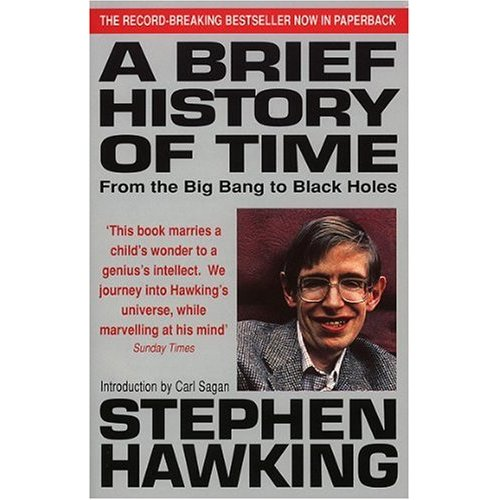
\includegraphics[width=6cm]{briefhist}
\end{center}
\end{column}
\begin{column}{6cm}
\begin{center}
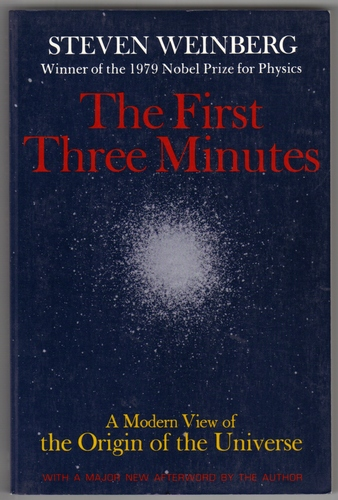
\includegraphics[width=4cm]{firstthree}
\end{center}
\end{column}
\end{columns}
\end{frame}

\begin{frame}
\frametitle{Initial interest (Cont'd)}
{\color{blue}Amazed by the cyclotron} studied in school:
\begin{center}
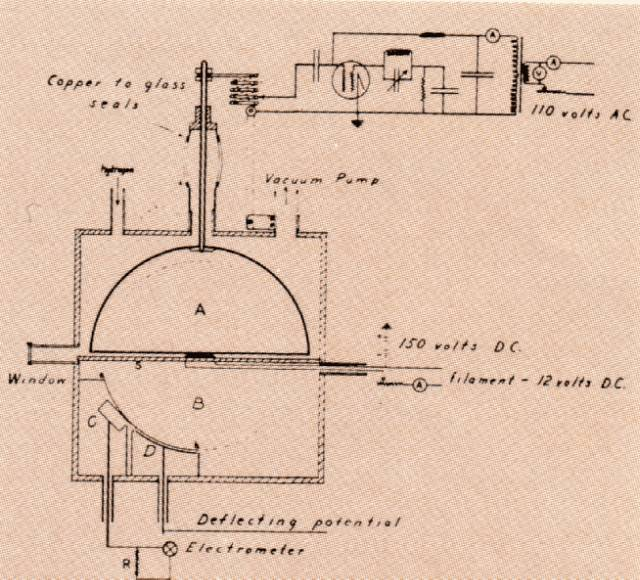
\includegraphics[width=6cm]{firstcyclo}
\end{center}
Wanted to work on accelerator physics, and make new discoveries\ldots\\
\begin{center} 
\alert{Decided to study high energy physics!}
\end{center}
\end{frame}

\begin{frame}
\frametitle{Initial interest (Cont'd)}
University curriculum:
\begin{itemize}
  \item First 2 years in Aix-en-Provence, 
  \item Then had to {\color{blue} move to Marseille} for the rest: Universit\'e
  de la M\'editerrann\'ee
  \item {\color{blue} Discovered CPPM} during first trip to University
  \begin{center}
  
\includegraphics[width=2cm]{logocppm}
  \end{center}
  \item Knew I would do my \alert{PhD. thesis there} \pause
  \item Managed to do that
\end{itemize}
\end{frame}

\part{PhD.: Flavour tagging in LHCb}
\begin{frame}
\partpage
\end{frame}
\begin{frame}
\frametitle{PhD.: the origins}
\begin{itemize}
  \item Started studying \alert{flavour tagging} between Licence and Master,
  with O.~Leroy in the {\color{blue} LHCb group at CPPM}.
  \item Internship at \alert{CERN in summer 2005}: Flavour tagging in Panoramix
  \item Master's {\color{blue} internship with O.~Leroy}: Study of secondary
  vertex reconstruction for flavour fagging in LHCb
  \item \alert{Accepted as PhD. student} under direction of R.~Le~Gac in the
  LHCb group of CPPM
\end{itemize}
\end{frame}

\begin{frame}
\frametitle{PhD.: the subject}
Title: Calibration of the flavour tagging algorithm of the LHCb experiment by
the measurement of $\sin(2\beta)$\\
~\\
\begin{itemize}
  \item Selection of control channels: $\PBu\to\PJpsi\PKplus$ and
  $\PBd\to\PJpsi\PKstar^0$
  \item Measurement of the mistag fraction using $\PBd$ mixing property
  \item Measurement of $\sin(2\beta)$ in $\PBd\to\PJpsi\PKshort$ using
  previously measured mistag rate, systematics' studies
\end{itemize}
\begin{columns}[t]
\begin{column}[T]{4cm}
\begin{block}{$\PBu\to\PJpsi\PKplus$}
1\,245 k events per year\\
$B/S = 1.6\pm0.2$
\end{block}
\end{column}
\begin{column}[T]{4cm}
\begin{block}{Mistag fraction}
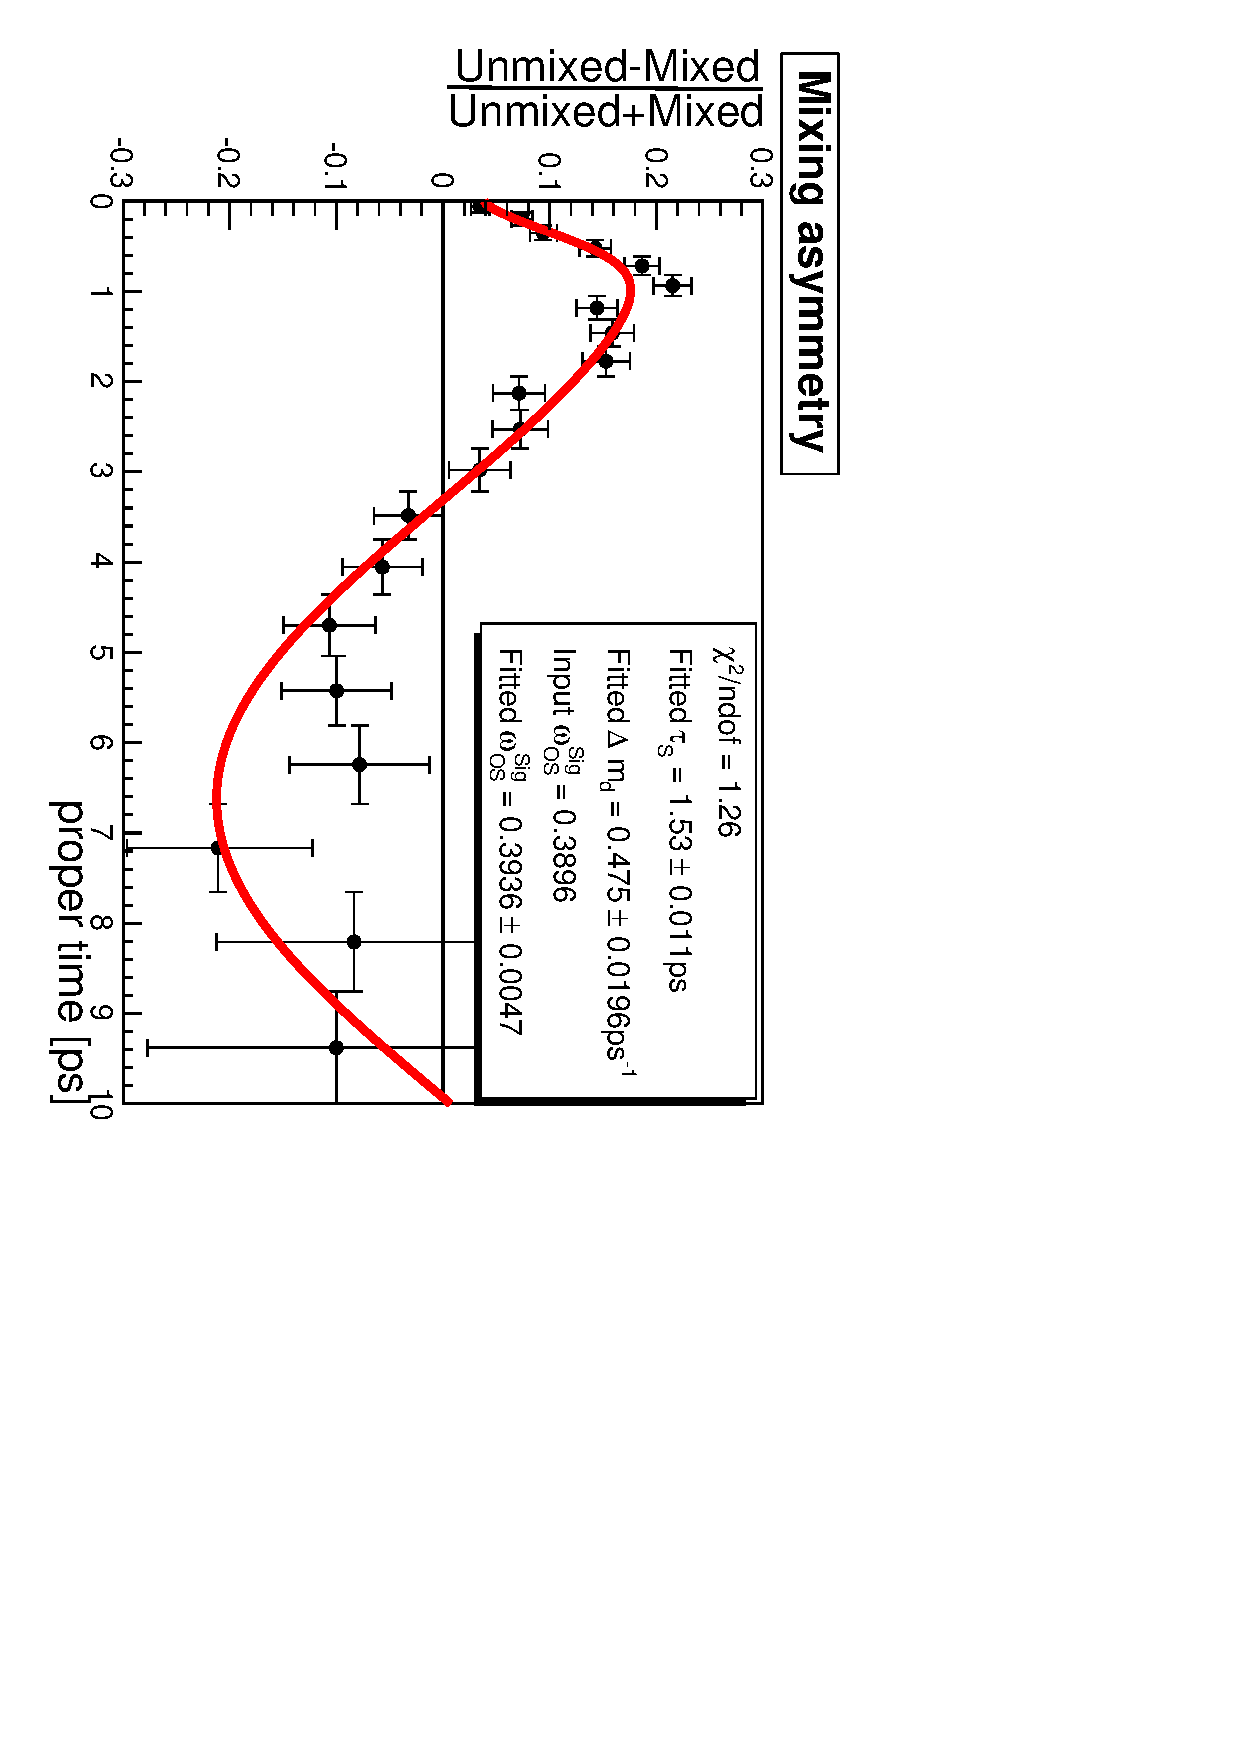
\includegraphics[angle=90,width=4cm]{CombinedAsymFit}
\end{block}
\end{column}
\begin{column}[T]{4cm}
\begin{block}{$\sin(2\beta)$}
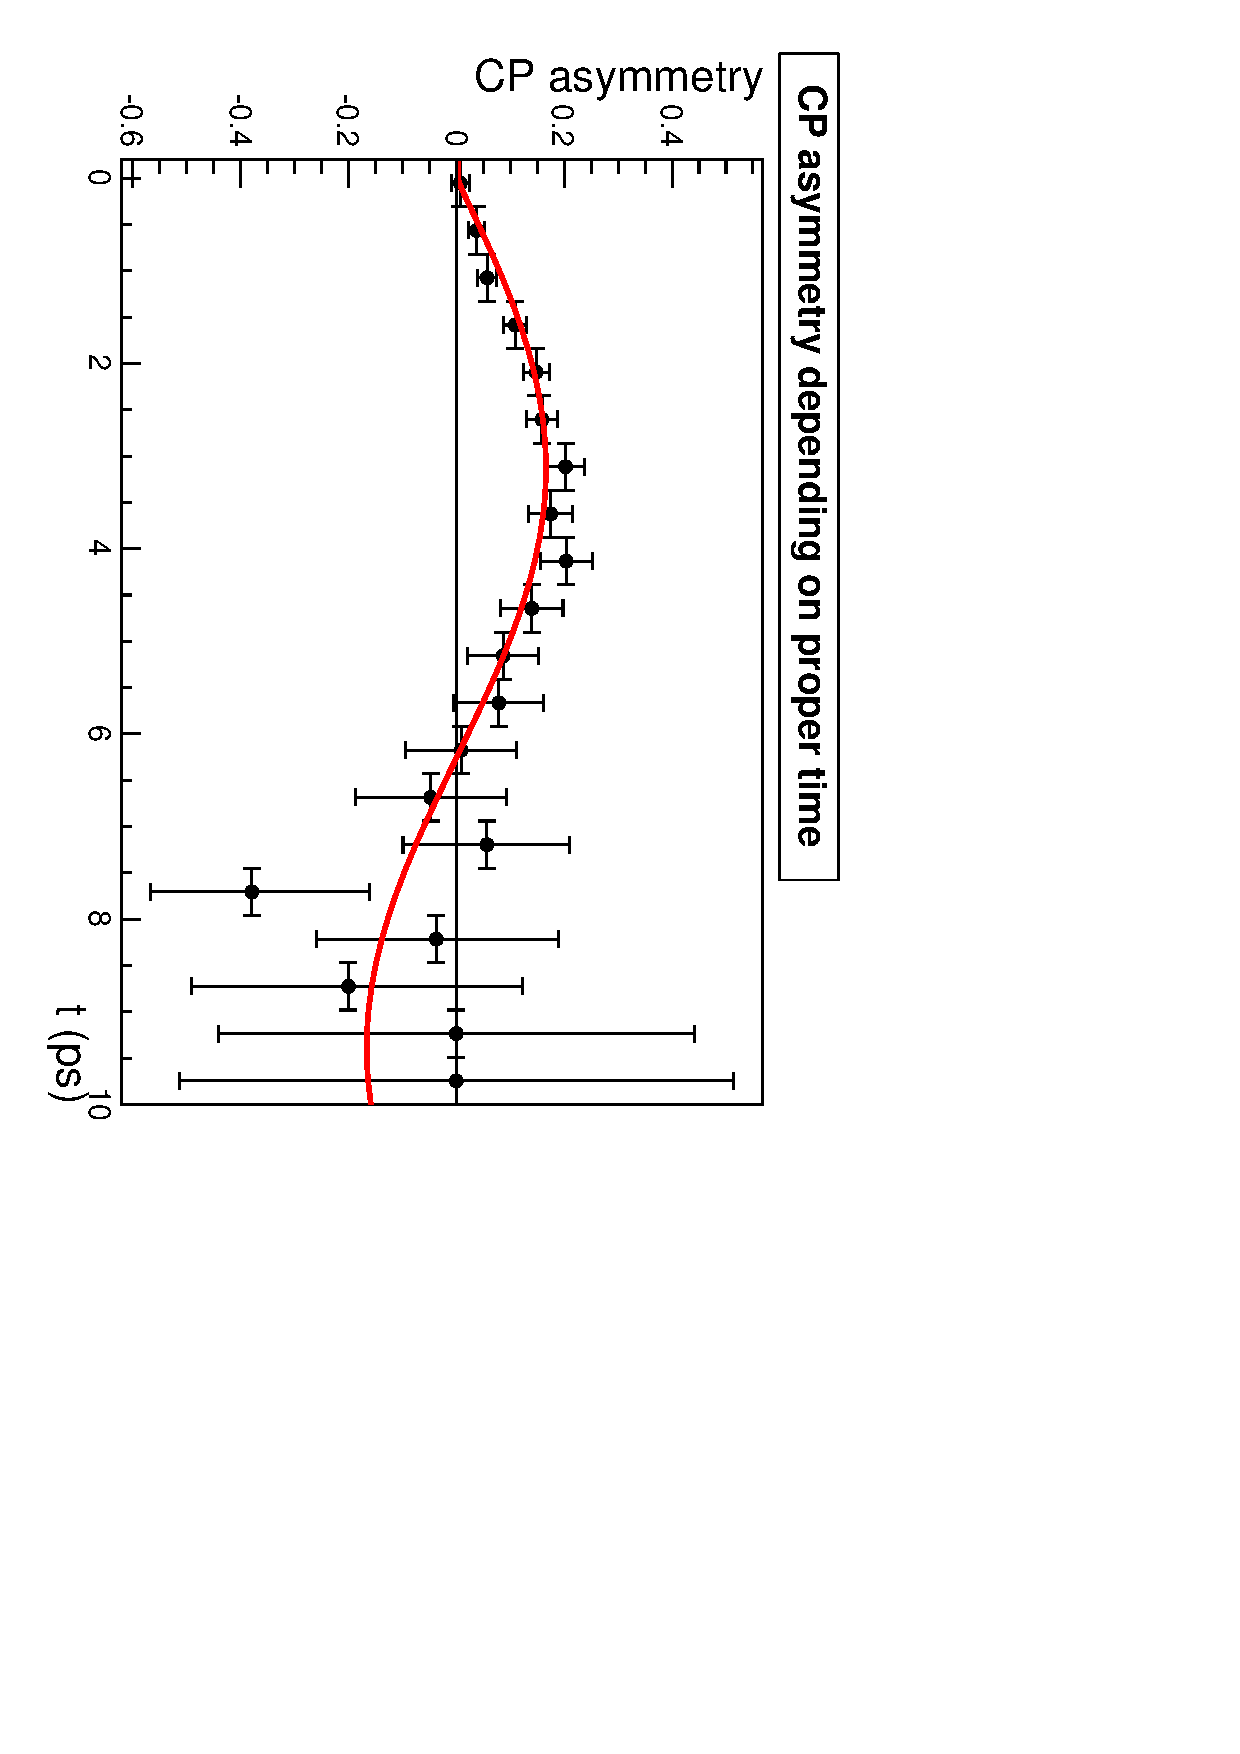
\includegraphics[angle=90,width=4cm]{AsymCPDC06AverageOmega}
\end{block}
\end{column}
\end{columns}
\end{frame}

\begin{frame}
\frametitle{PhD.: Using DIRAC in LHCb}
Several {\color{blue}millions of events} to analyse + {\color{blue}thousands of
toy MC studies}: used DIRAC a lot.
\begin{center}
here figure
\end{center}
I wanted to \alert{continue working with this tool}.
\end{frame}

\part{CERN fellowship}
\begin{frame}
\partpage
\end{frame}
\begin{frame}
\frametitle{The project}
\begin{itemize}
  \item Applied for \alert{fellowship at CERN}, emphasis on {\color{blue}DIRAC
  in LHCb}
  \item Contacted by L. Linssen ({\color{blue}LCD group}) to develop a
  \alert{DIRAC instance for the ILC~VO}:\\ 
  \begin{itemize}  
    \item Aim is \alert{mass production of Monte Carlo data} for the CLIC
    Conceptual Design Report (CDR): {\color{blue}benchmark of 2 detector
    concepts} (ILD and SiD)
  \end{itemize}
  \item Running productions
\end{itemize}
\end{frame}

\begin{frame}
\frametitle{The ILCDIRAC instance}
The need of a {\color{blue}production system for the CDR} made the LCD group
turn towards DIRAC, well proven solution from LHCb.\\
ILCDIRAC: DIRAC instance dedicated to the {\color{blue}linear collider
community}:
\begin{itemize}
  \item Specific interface to handle ILC applications: 6 different types with
  different user interfaces
  \item More than {\color{blue}2 million jobs processed in 1 year}: CLIC CDR
  production and user jobs
  \item Users not only at CERN, but also LAL (Fr.), MPI (De.), VINCA (R.S.),
  etc.
  \item {\color{blue}Adopted by the SiD detector concept} as the official
  production system for the next ILC document: the DBD.
\end{itemize}

\end{frame}

\part{Current duties}
\begin{frame}
\partpage
\end{frame}
\begin{frame}
\frametitle{Current duties}
ILCDIRAC management:
\begin{itemize}
  \item Development of \alert{new features}
  \item \alert{Monitoring} of VOBOX status
  \item {\color{blue}Installation and setup} of services
  \item Interaction with storage
\end{itemize}
Mass Production:
\begin{itemize}
  \item Generator: setup of applications, registration of new process; tests
  \item \alert{Production manager}: definition of new productions, monitor
  statuses, produce statistics
  \item Data manager: make sure the data is where it's supposed to be, replicate
  when needed, check availability of resources
\end{itemize}
\end{frame}

\begin{frame}
\frametitle{Current duties (Cont'd)}
Other:
\begin{itemize}
  \item $\Ptop\APtop$ at 500GeV analysis convener: one of the 6 benchmark
  channels for the CLIC detectors, small group
  \item LCD group computing coordinator: who has which computer? Who needs one?
  \item Student supervision: P.~Majewski, E.~Hidle and C.~B.~Lam
\end{itemize}
\end{frame}
 
\part{Conclusion}
\begin{frame}
\partpage
\end{frame}
\begin{frame}
\frametitle{Conclusion} 
\begin{itemize}
  \item \alert{I'm a physicist}\pause
  \item with {\color{blue}computing interest}, in particular \alert{DIRAC}\pause
  \item Changing experiment was very interesting\pause
  \item Developing ILCDIRAC implied \alert{looking deeply into DIRAC}: service
  and agents, configuration, etc.\pause
  \item Ready to take responsibilities
\end{itemize}
\end{frame}
\end{document}